% =============================================================================
% COPYRIGHT AND DISCLAIMER
% =============================================================================
% This file is provided as a convenience template for competition participants.
% By using it, you accept full responsibility for compliance with all applicable
% copyright, licensing, and usage rules of the Association for Computing
% Machinery (ACM) and of any LaTeX packages you load (including, without
% limitation, the "acmart" document class and related ACM materials).
%
% Consult ACM's official publication, template, and copyright policies before
% using this setup for any purpose other than this competition. Do not assume
% that this template may be reused, redistributed, or submitted elsewhere
% without independently verifying ACM's current rules.
%
% Use of the "acmart" class, the "sigconf" option, or ACM-style formatting in
% this template does NOT mean that this report, this competition, its organizers,
% or any resulting PDF is sponsored, endorsed, affiliated with, or published by
% ACM. ACM trademarks and branding remain the property of ACM.
%
% Template packages live in preamble.tex.
% Citations live in main.bib. Edit this file with your paper content.
% =============================================================================

\documentclass[sigconf]{acmart}
% =============================================================================
% Template setup — participants normally do not edit this file.
% Author content belongs in main.tex; citations belong in main.bib.
% \documentclass lives in main.tex so Overleaf does not treat this file as root.
% =============================================================================

% --- Competition / non-ACM-submission friendly rights metadata -------------
\setcopyright{none}
\settopmatter{printacmref=false}
\acmConference[Kaggle Competition]{Filament Segmentation Challenge}{2026}{\href{https://www.kaggle.com/competitions/filament-segmentation-2026}{kaggle.com/competitions/filament-segmentation-2026}}
\acmBooktitle{Competition Report}
\acmDOI{}
\acmISBN{}

% --- Author guidance text --------------------------------------------------
% \guide{...} is gray italic while \guideStyletrue; omitted from the PDF if false.
% Flip the switch in main.tex after % =============================================================================
% Template setup — participants normally do not edit this file.
% Author content belongs in main.tex; citations belong in main.bib.
% \documentclass lives in main.tex so Overleaf does not treat this file as root.
% =============================================================================

% --- Competition / non-ACM-submission friendly rights metadata -------------
\setcopyright{none}
\settopmatter{printacmref=false}
\acmConference[Kaggle Competition]{Filament Segmentation Challenge}{2026}{\href{https://www.kaggle.com/competitions/filament-segmentation-2026}{kaggle.com/competitions/filament-segmentation-2026}}
\acmBooktitle{Competition Report}
\acmDOI{}
\acmISBN{}

% --- Author guidance text --------------------------------------------------
% \guide{...} is gray italic while \guideStyletrue; omitted from the PDF if false.
% Flip the switch in main.tex after % =============================================================================
% Template setup — participants normally do not edit this file.
% Author content belongs in main.tex; citations belong in main.bib.
% \documentclass lives in main.tex so Overleaf does not treat this file as root.
% =============================================================================

% --- Competition / non-ACM-submission friendly rights metadata -------------
\setcopyright{none}
\settopmatter{printacmref=false}
\acmConference[Kaggle Competition]{Filament Segmentation Challenge}{2026}{\href{https://www.kaggle.com/competitions/filament-segmentation-2026}{kaggle.com/competitions/filament-segmentation-2026}}
\acmBooktitle{Competition Report}
\acmDOI{}
\acmISBN{}

% --- Author guidance text --------------------------------------------------
% \guide{...} is gray italic while \guideStyletrue; omitted from the PDF if false.
% Flip the switch in main.tex after \input{preamble}.
%
% Do not use \guide{...} for \email{...}.
\usepackage{xcolor}
\newif\ifguideStyle
\guideStyletrue
\newcommand{\guide}[1]{%
  \ifguideStyle
    {\color{gray!65}\itshape #1}%
  \fi
}

% --- Math ------------------------------------------------------------------
% Do NOT load amssymb (or amsfonts): acmart already loads newtxmath, which
% defines the same symbols (e.g. \Bbbk) and causes a conflict on Overleaf.
% amsmath is already provided by acmart; mathtools extends it.
\usepackage{mathtools}

% --- Figures ---------------------------------------------------------------
% graphicx is already loaded by acmart
\usepackage{subcaption}

% --- Tables ----------------------------------------------------------------
% booktabs is already loaded by acmart
\usepackage{tabularx}
\usepackage{multirow}

% --- Bibliography style is set in main.tex (ACM-Reference-Format) ----------
.
%
% Do not use \guide{...} for \email{...}.
\usepackage{xcolor}
\newif\ifguideStyle
\guideStyletrue
\newcommand{\guide}[1]{%
  \ifguideStyle
    {\color{gray!65}\itshape #1}%
  \fi
}

% --- Math ------------------------------------------------------------------
% Do NOT load amssymb (or amsfonts): acmart already loads newtxmath, which
% defines the same symbols (e.g. \Bbbk) and causes a conflict on Overleaf.
% amsmath is already provided by acmart; mathtools extends it.
\usepackage{mathtools}

% --- Figures ---------------------------------------------------------------
% graphicx is already loaded by acmart
\usepackage{subcaption}

% --- Tables ----------------------------------------------------------------
% booktabs is already loaded by acmart
\usepackage{tabularx}
\usepackage{multirow}

% --- Bibliography style is set in main.tex (ACM-Reference-Format) ----------
.
%
% Do not use \guide{...} for \email{...}.
\usepackage{xcolor}
\newif\ifguideStyle
\guideStyletrue
\newcommand{\guide}[1]{%
  \ifguideStyle
    {\color{gray!65}\itshape #1}%
  \fi
}

% --- Math ------------------------------------------------------------------
% Do NOT load amssymb (or amsfonts): acmart already loads newtxmath, which
% defines the same symbols (e.g. \Bbbk) and causes a conflict on Overleaf.
% amsmath is already provided by acmart; mathtools extends it.
\usepackage{mathtools}

% --- Figures ---------------------------------------------------------------
% graphicx is already loaded by acmart
\usepackage{subcaption}

% --- Tables ----------------------------------------------------------------
% booktabs is already loaded by acmart
\usepackage{tabularx}
\usepackage{multirow}

% --- Bibliography style is set in main.tex (ACM-Reference-Format) ----------


% Guide styling: \guideStyletrue = show gray italic hints; \guideStylefalse = omit them
% \guideStyletrue
\guideStylefalse

\begin{document}

\title{Multi-Scale Mask Refinement and Disjoint Instance Scoring for Solar Filament Segmentation}
\subtitle{A Solution to the Solar Filament Segmentation Challenge 2026} % DO NOT CHANGE


\author{Adam Pipal}
\affiliation{%
  \institution{Independent Researcher}
  \city{Prague}
  \country{Czech Republic}
}
\email{adampipal22@gmail.com}

\begin{abstract}
    This report describes our solution to the Solar Filament Segmentation Challenge~2026, a Kaggle competition on automatic segmentation of solar filaments in GONG H-$\alpha$ observations. Our pipeline combines a six-family Mask~R-CNN proposal ensemble (30~checkpoints evaluated across four flip views via Weighted Mask Fusion), full-disk \texttt{ResNet50} and \texttt{ResNeXt101} semantic U-Net priors, dual target-aligned ROI boundary refiners (\texttt{ResidualCropRefinerUNet} and wide-context \texttt{WideContextRefinerUNetV2}), a 25-booster 5-fold cross-fitted LightGBM ranker, and greedy pixel-disjoint canvas painting. Across strict observation-grouped 5-fold cross-validation over all 707 training observations (1,154 annotator records; 8,199 ground-truth filaments), nested refinement and scoring lift pooled Panoptic Quality (PQ) from \textbf{0.4521} \texttt{[nested]} / \textbf{0.4543} \texttt{[in-sample]} (Rule~B, Public LB \textbf{0.40}) to \textbf{0.4688} \texttt{[nested]} (Rule~C / Phase~3B Local, $\text{SQ}=0.6857$, $\text{RQ}=0.6836$, paired bootstrap $P=1.000$, Public LB \textbf{0.41}), with zero pixel overlaps across predicted instances and all 81 FP16 checkpoints stored in-repo ($<100\text{ MB}$ each).
\end{abstract}

\maketitle

\ifguideStyle
\noindent{\color{gray!65}\itshape
Guide mode is on.}
\par\medskip
\fi

% ==================================== %
%              INTRODUCTION            %
% ==================================== %
\section{Introduction}
    This report goes over the details of our submitted solution to the Solar Filament Segmentation Challenge~2026 \cite{filament-segmentation-2026}. The challenge, launched on July~10,~2026, is organized by the Earth-Space AI Research (ESAIR) Lab\footnote{\href{https://www.esairlab.com/home}{www.esairlab.com/}}. This challenge utilizes the MAGFiLO dataset for evaluation of the segmentation algorithms \cite{ahmadzadeh2024dataset}. Our reproducible codebase and model weights are released at \url{https://github.com/Harru230/solar}.

    Segmenting filaments in $2048\times 2048$ H-$\alpha$ filtergrams presents three primary failure modes: extreme aspect ratios and thin ($<5\text{ px}$) structures lost under coarse $28\times 28$ RoI mask heads, boundary discretization mismatches relative to COCO vector polygon targets, and inter-annotator variance across partially overlapping or fragmented threads. We address these via multi-resolution detection diversity, full-frame plus ROI boundary refinement trained directly on official \texttt{frPyObjects} targets, and non-drifting cross-fitted instance selection.


% ==================================== %
%              METHODOLOGY             %
% ==================================== %
\section{Methodology}\label{sec:methodology}
    Figure~\ref{fig:pipeline} illustrates the complete end-to-end architecture. Every stage respects strict observation-level 5-fold grouped cross-validation (142/142/141/141/141 observations) balanced by observatory code, preventing any leakage across multi-annotator records.

\begin{figure*}[t]
    \centering
    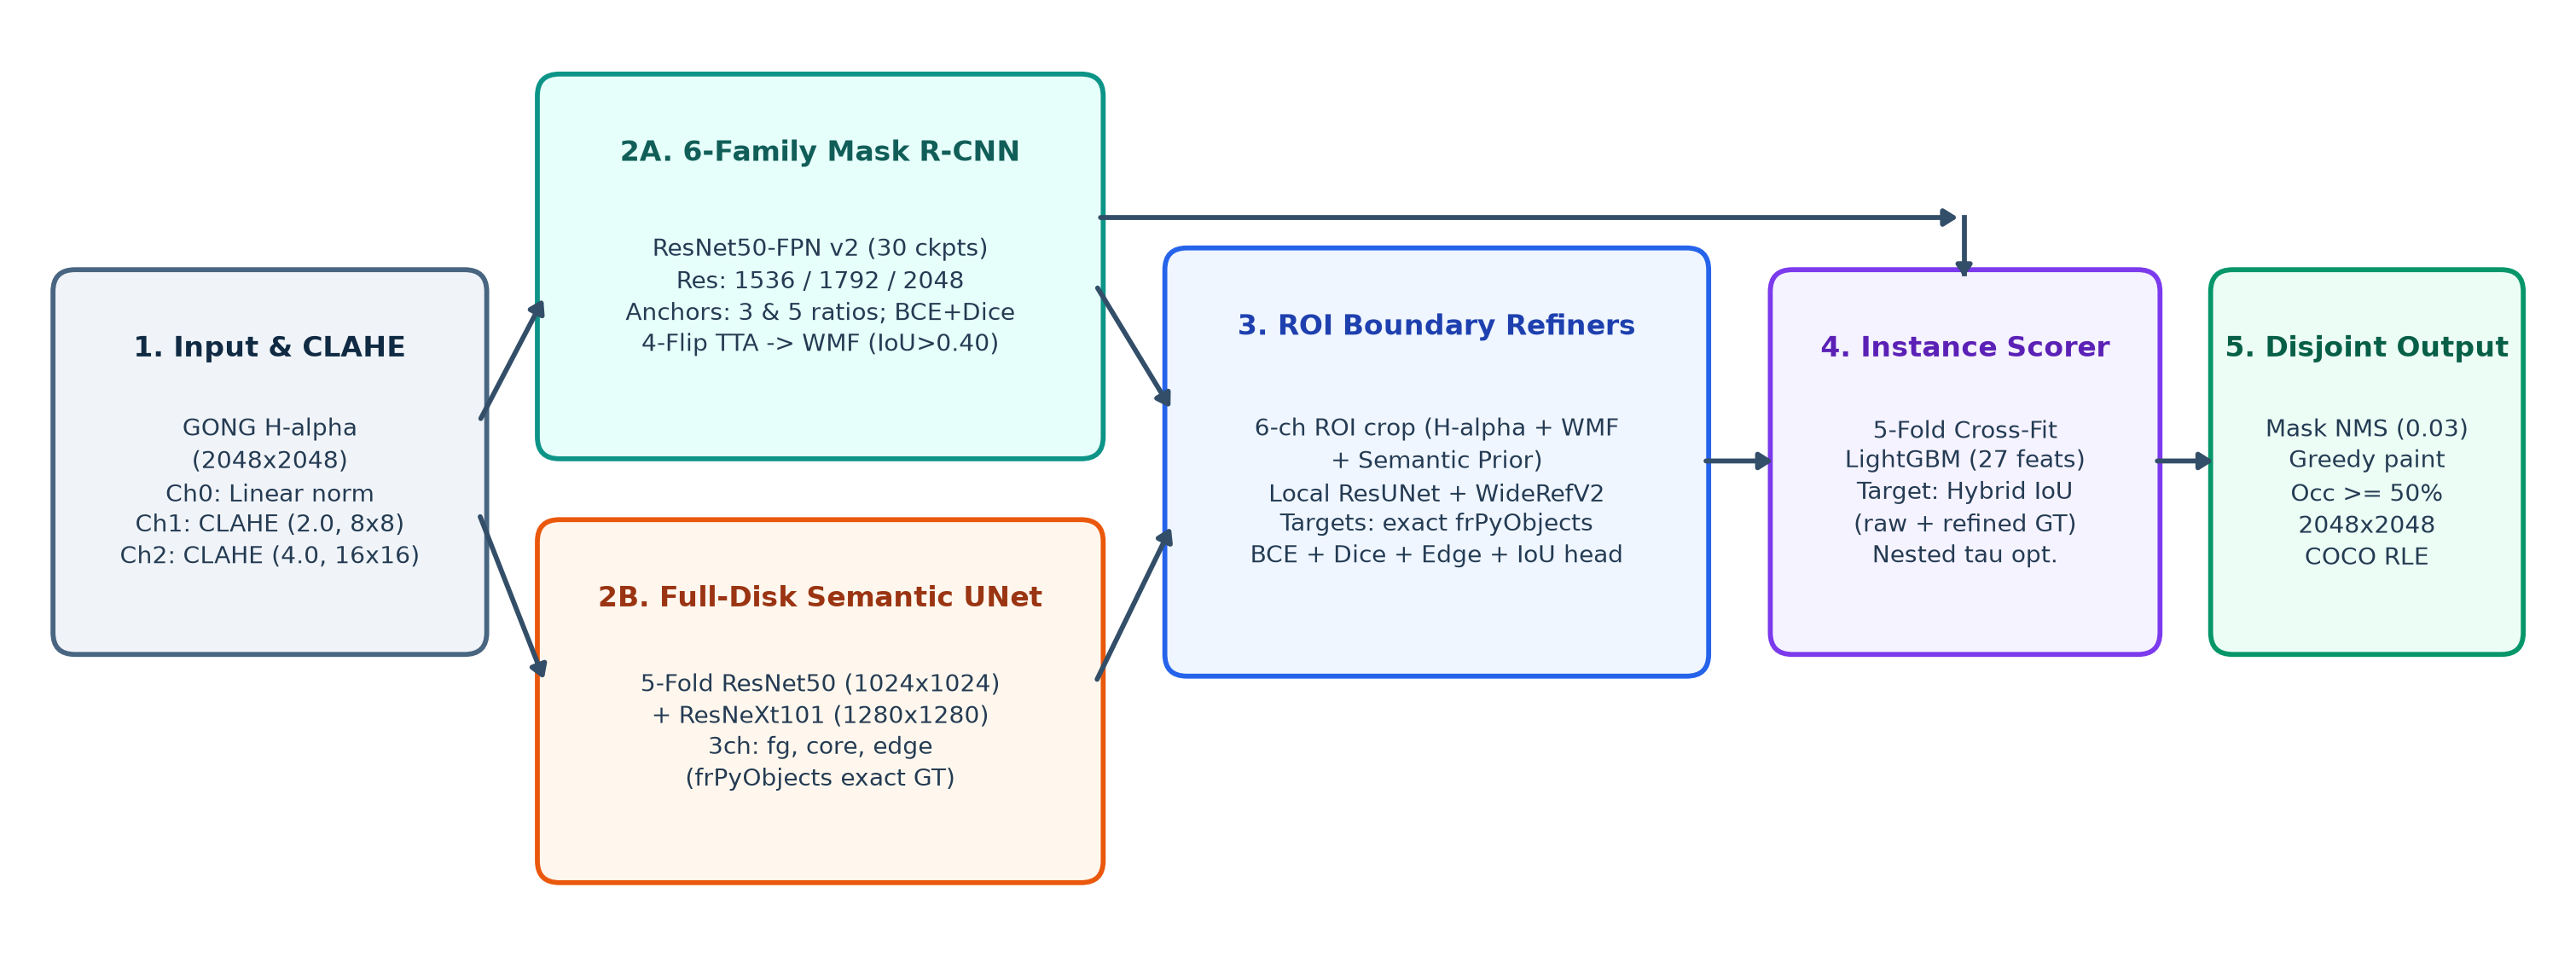
\includegraphics[width=0.95\textwidth]{figures/pipeline_diagram.png}
    \caption{End-to-end pipeline: deterministic multi-scale CLAHE preprocessing feeds a 30-checkpoint Mask~R-CNN proposal ensemble and full-disk semantic U-Nets, followed by \texttt{frPyObjects}-aligned ROI boundary refinement, LightGBM scoring, and pixel-disjoint painting.}
    \label{fig:pipeline}
\end{figure*}

    \subsection{Preprocessing and Validation Split}
    Raw $2048\times 2048$ grayscale H-$\alpha$ images are mapped deterministically to three channels: linear intensity $I/255$, fine CLAHE (clip limit $2.0$, $8\times 8$ tiles), and coarse CLAHE ($4.0$, $16\times 16$). The 707 training observations (1,154 annotator records; 296 multi-annotator observations; 8,199 ground-truth polygons) are split into five observation-disjoint folds; median nearest-neighbor temporal separation is $46.4\text{ h}$ in CV versus $36.7\text{ h}$ between test (180 images) and training data.

    \subsection{Multi-Family Detection \& Weighted Mask Fusion}
    We fine-tune six Mask~R-CNN (\texttt{ResNet50-FPN v2}) families \cite{he2017mask,he2016deep} across all 5~folds (30 checkpoints total; 30~epochs AdamW, \texttt{bfloat16} AMP training, mandatory strict \texttt{float32} inference): \texttt{clahe} ($1536$, 3~anchors, BCE), \texttt{anchors5} ($1536$, 5~anchors, BCE), \texttt{dice} ($1536$, 3~anchors, BCE+Soft Dice), \texttt{a5dice} ($1536$, 5~anchors, BCE+Soft Dice), \texttt{1792\_clahe} ($1792$, 3~anchors, BCE), and \texttt{2048} ($2048$, 3~anchors, BCE). Each model runs 4-flip TTA (\texttt{id, h, v, hv} = 24 views/image in OOF; 120 in test). Proposals $\ge 0.25$ are rescaled as $\tilde{s}_i = s_i^\gamma w_{\text{fam}(i)}$ ($w=2.0$ for \texttt{2048}/\allowbreak\texttt{1792\_clahe}, $\gamma=1.5$ in Rule~B) and greedily clustered ($\text{mask IoU} > 0.40$) into soft probability maps $\bar{P}_c$. All candidates with cluster score $\ge 0.20$ enter the refinement pool (7,803 OOF; 2,074 test).

    \subsection{Semantic Priors and Target-Aligned Refiners}
    While Mask~R-CNN excels at localization, its $28\times 28$ RoI head thickens predictions (10.6~px vs 8.3~px GT width) and leaves fine boundaries blurred relative to \texttt{pycocotools} \texttt{frPyObjects} polygon masks used by official evaluation:
    \begin{itemize}
        \item \textbf{Full-Disk Semantic U-Nets}: Five-fold \texttt{ResNet50} ($1024^2$, 2~channels) and \texttt{ResNeXt101} ($1280^2$, 3~channels) \cite{xie2017aggregated,ronneberger2015u} backbones predict foreground, filament core, and boundary edge maps directly against union \texttt{frPyObjects} targets across the solar disk.
        \item \textbf{Dual ROI Boundary Refiners}: Five-fold cross-fitted \texttt{Residual\allowbreak CropRefinerUNet} ($160^2$, $\text{pad}=12$, 6~channels) and ResSE-ASPP \texttt{WideContext\allowbreak RefinerUNetV2} ($224^2$, $\text{pad}=56$, 11~channels incorporating neighbor suppression and both semantic priors) predict \texttt{frPyObjects}-aligned masks and IoU scores, blended via \texttt{wref\_\allowbreak uv1\_t50} ($\tau_{\text{mask}}=0.50$).
    \end{itemize}

    \subsection{Cross-Fitted Scoring \& Pixel-Disjoint Painting}
    Using 27 view- and refiner-derived geometric, intensity, and agreement features, a 25-booster 5-fold cross-fitted \texttt{LightGBM} ranker \cite{ke2017lightgbm} (\texttt{LGB\_S27\_yhyb}, 5~seeds $\times$ 5~folds) predicts hybrid GT IoU. Candidates sorted descending undergo greedy mask NMS ($\text{IoU} \le 0.03$), refined mask blending, disjoint canvas subtraction ($\ge 10\text{ px}$, $\ge 50\%$ retained area), and COCO RLE encoding. Cutoffs $\tau$ ($\text{median } 0.255$) maximize nested 5-fold OOF PQ.

\begin{figure}[t]
    \centering
    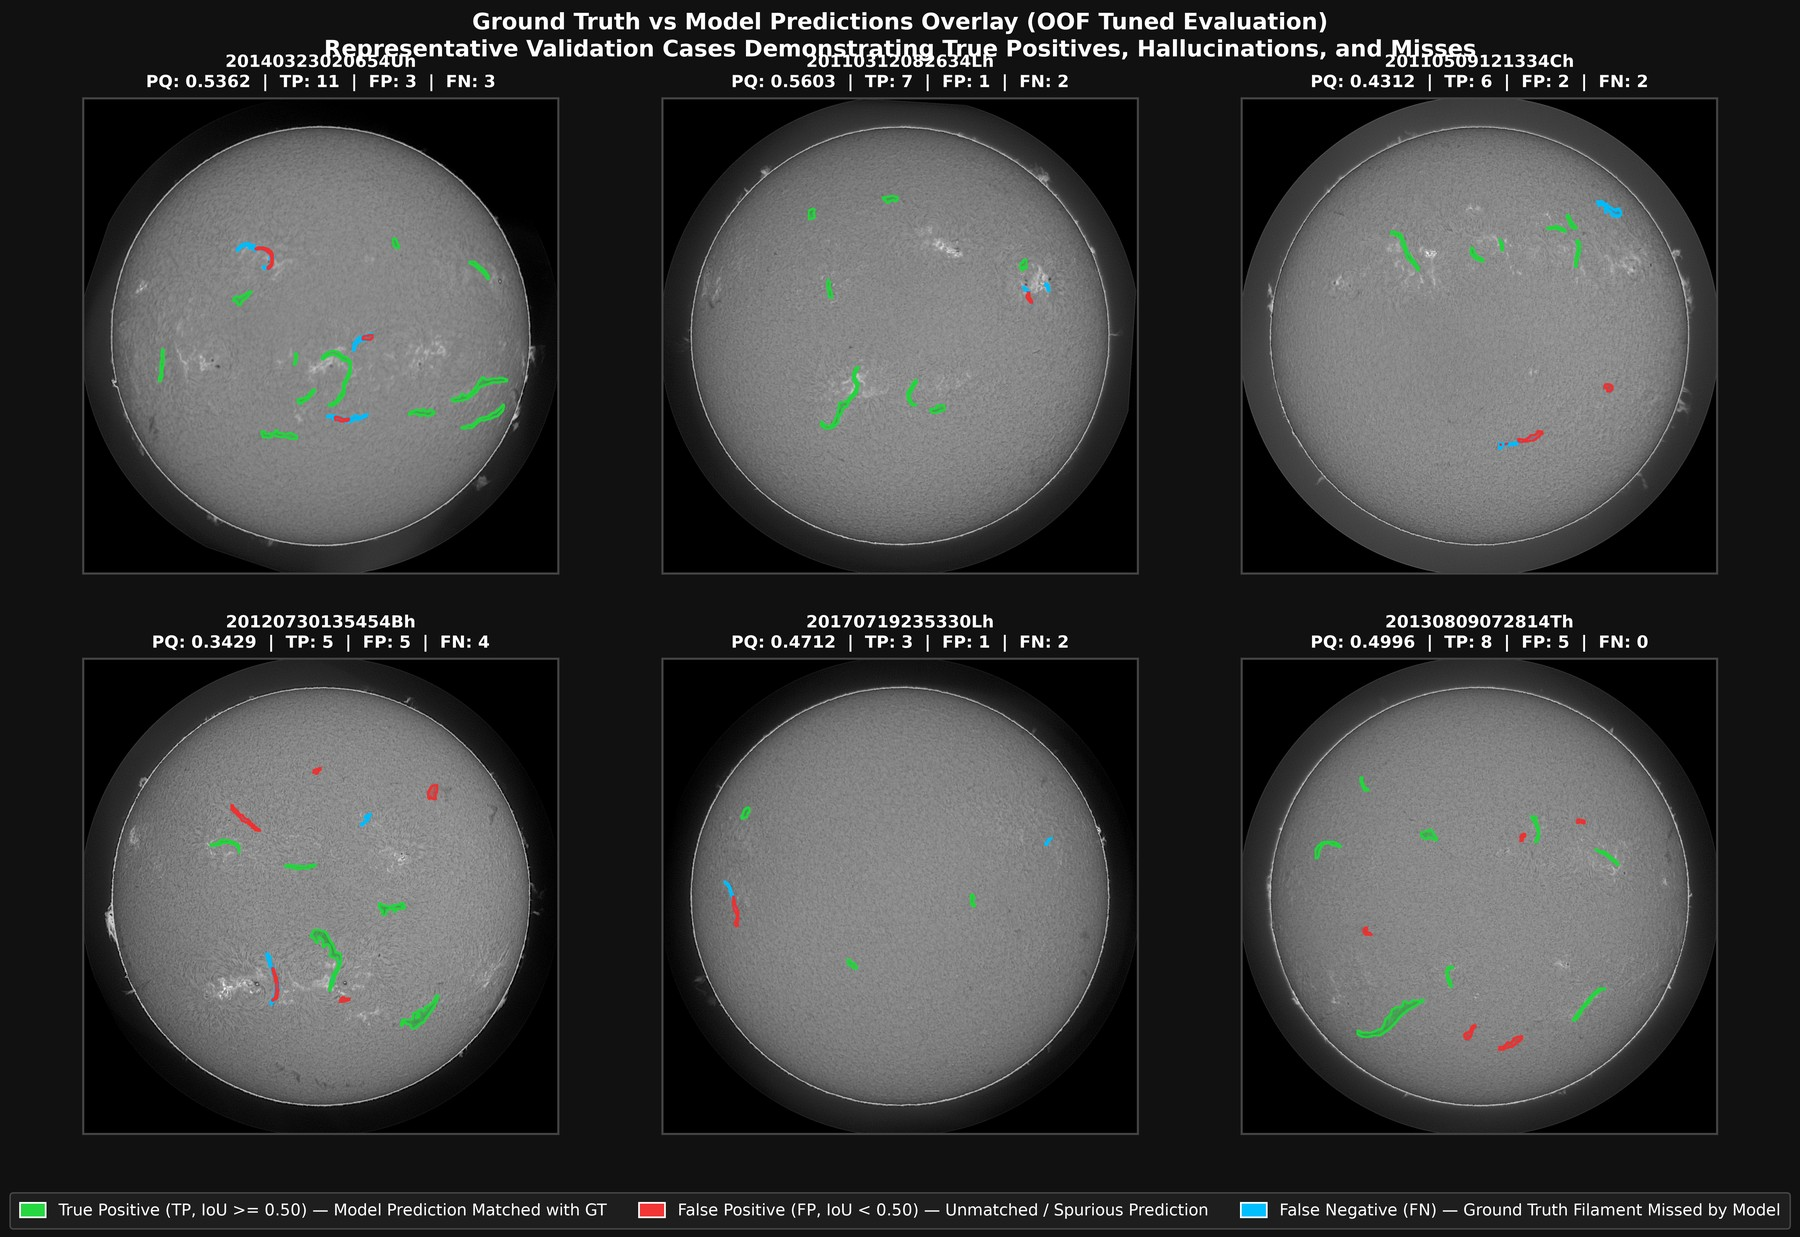
\includegraphics[width=\linewidth]{figures/gt_vs_pred_overlay.jpg}
    \caption{Qualitative full-disk H-$\alpha$ comparison showing human expert polygons (green/yellow), disjoint predicted filaments (cyan/blue), TPs, FPs, and missed thin threads.}
    \label{fig:qual}
\end{figure}


% ==================================== %
%              EVALUATION              %
% ==================================== %
\section{Evaluation}\label{sec:evaluation}
    All OOF scores follow the official competition engine (\texttt{pq\_eval.py}): each (annotator, observation) record is matched independently against unique predictions at $\text{IoU} > 0.50$, and $\text{PQ} = \text{SQ} \times \text{RQ}$ is pooled across all 707 observations (1,154 records, 8,199 GT masks).

\begin{table}[t]
    \caption{Progression across 5-fold OOF (707 obs, 1,154 records) and 180-image Test. Nested threshold $\tau$ is tuned strictly out-of-fold.}
    \label{tab:results}
    \centering
    \small
    \resizebox{\linewidth}{!}{%
    \begin{tabular}{@{}lcccc@{}}
        \toprule
        Configuration & Eval Tag & PQ & SQ / RQ & Preds (Test) \\
        \midrule
        Single \texttt{1536 clahe} (4-TTA) & \texttt{[in-sample]} & 0.4338 & 0.6687 / 0.6487 & — \\
        Single \texttt{2048 BCE} (4-TTA) & \texttt{[nested]} & 0.4400 & 0.6731 / 0.6537 & — \\
        6-Fam Rule A (Uniform WMF) & \texttt{[nested]} & 0.4508 & 0.6761 / 0.6668 & 1,165 (LB 0.39) \\
        6-Fam Rule B (Weighted WMF) & \texttt{[nested]} & 0.4521 & 0.6777 / 0.6672 & — \\
        6-Fam Rule B (Fixed Global) & \texttt{[in-sample]} & 0.4543 & 0.6773 / 0.6708 & 1,155 (LB 0.40) \\
        Phase 2 Local (\texttt{CropV1 + LGB}) & \texttt{[nested]} & 0.4676 & — & — \\
        \textbf{Phase 3B Local Winner (\texttt{Rule C})} & \texttt{[nested]} & \textbf{0.4688} & \textbf{0.6857 / 0.6836} & \textbf{1,170 (LB 0.41)} \\
        Hybrid A100 (\texttt{ConvNeXt V1 + S27}) & \texttt{[nested]} & 0.4692 & 0.6858 / 0.6841 & 1,182 (LB 0.40, cache) \\
        \bottomrule
    \end{tabular}%
    }
\end{table}

\begin{table}[t]
    \caption{707-image OOF distributions and matching audit (Rule~B \texttt{[in-sample]} baseline vs Phase~3B Local \texttt{Rule C} \texttt{[nested]}).}
    \label{tab:distributions}
    \centering
    \small
    \resizebox{\linewidth}{!}{%
    \begin{tabular}{@{}lcccc@{}}
        \toprule
        Metric (707 OOF Images) & Mean $\pm$ Std & Median & [p25, p75] & Tail / Note \\
        \midrule
        Per-Image PQ (Rule~B, \texttt{[in-sample]}) & $0.4457 \pm 0.1494$ & 0.4585 & [0.374, 0.543] & max 0.8072 \\
        Per-Image Union Dice (Rule~B, \texttt{[in-sample]}) & $0.6541 \pm 0.1570$ & 0.6887 & [0.603, 0.753] & p95 0.8110 \\
        Per-Image Union Dice (\texttt{Rule C}, \texttt{[nested]}) & \textbf{0.6639} & \textbf{0.7002} & — & $k=1$ mean 0.6557 \\
        Per-Image Union IoU (Rule~B, \texttt{[in-sample]}) & $0.5044 \pm 0.1465$ & 0.5265 & [0.434, 0.605] & p95 0.6821 \\
        Matched TP Inst IoU (Rule~B, \texttt{[in-sample]}) & 0.6773 & 0.6808 & [0.615, 0.744] & max 0.907 \\
        Matched TP Inst IoU (\texttt{Rule C}, \texttt{[nested]}) & \textbf{0.6857} & \textbf{0.6911} & — & TP 5,344 / FP 2,091 \\
        Matched TP Inst Dice (Rule~B, \texttt{[in-sample]}) & 0.8045 & 0.8101 & [0.761, 0.853] & max 0.951 \\
        GT Split / Pred Merge ($\text{IoU}>0.15$, \texttt{Rule C}) & 1.32\% / 1.60\% & — & — & GT multi-hit 0\% (A/B) \\
        Pred multi-hit ($\text{IoU}>0.5$, Rule~B) & 1 / 7,497 (0.013\%) & — & — & bridge 2.84\% ($\text{IoU}>0$) \\
        \bottomrule
    \end{tabular}%
    }
\end{table}

    \subsection{Quantitative Gain, Uncertainty \& Drift Checks}
    Table~\ref{tab:results} summarizes progression: full Phase~3B local refinement (\texttt{Rule C}, \texttt{wref\_\allowbreak uv1\_t50}) lifts pooled \texttt{[nested]} PQ by \textbf{+0.0166} over \texttt{[nested]} Rule~B ($0.4521 \rightarrow 0.4688$) and by \textbf{+0.0144} over \texttt{[in-sample]} Rule~B ($0.4543 \rightarrow 0.4688$; $\text{TP}=5{,}344, \text{FP}=2{,}091, \text{FN}=2{,}855$, single-annotator $k=1$ PQ $0.4720$, multi $0.4668$), and by $+0.0012$ ($P=0.9677$) over Phase~2 Local. An auxiliary external-cache \texttt{ConvNeXt\allowbreak AttnRefinerNet} hybrid reaches $0.4692$ \texttt{[nested]} ($\text{SQ}=0.6858, \text{RQ}=0.6841$, Public LB $0.40$) but is omitted in favor of \texttt{Rule C} (Public LB \textbf{0.41}) to guarantee 100\% self-contained in-repo FP16 checkpoint reproducibility; Stage-2 uncovered-filament recovery yielded no significant net PQ gain and was likewise omitted. Across 10,000 image-level bootstrap resamples, the \texttt{Rule C} gain over Rule~B is decisive ($P=1.000$, 95\% CI $[+0.0114, +0.0175]$). Figures~\ref{fig:error_morph}--\ref{fig:matching_err} show baseline distributions, morphology stratification, and matching errors; adversarial OOF-vs-Test LightGBM AUC is $0.5077$ on detector features and $0.6206$ on S27 features (multiplicity ratio $1.008\times$: $1{,}170/180$ vs $4{,}559/707$, primary-scale KS $p \ge 0.538$ and all 15 morphological metrics $p \ge 0.051$). Regenerating all 180 test images in strict \texttt{FP32} from the 81 in-repo \texttt{FP16} checkpoints confirms parity against the Kaggle CSVs (mean union/instance IoU \textbf{0.961}/\textbf{0.970} for the single Selected final submission \texttt{submission\_phase3b\_local.csv}, and $0.943/0.957$, $0.932/0.954$ for Rule~B/A ablations relative to the original \texttt{bfloat16}-cached baseline).

\begin{figure}[t]
    \centering
    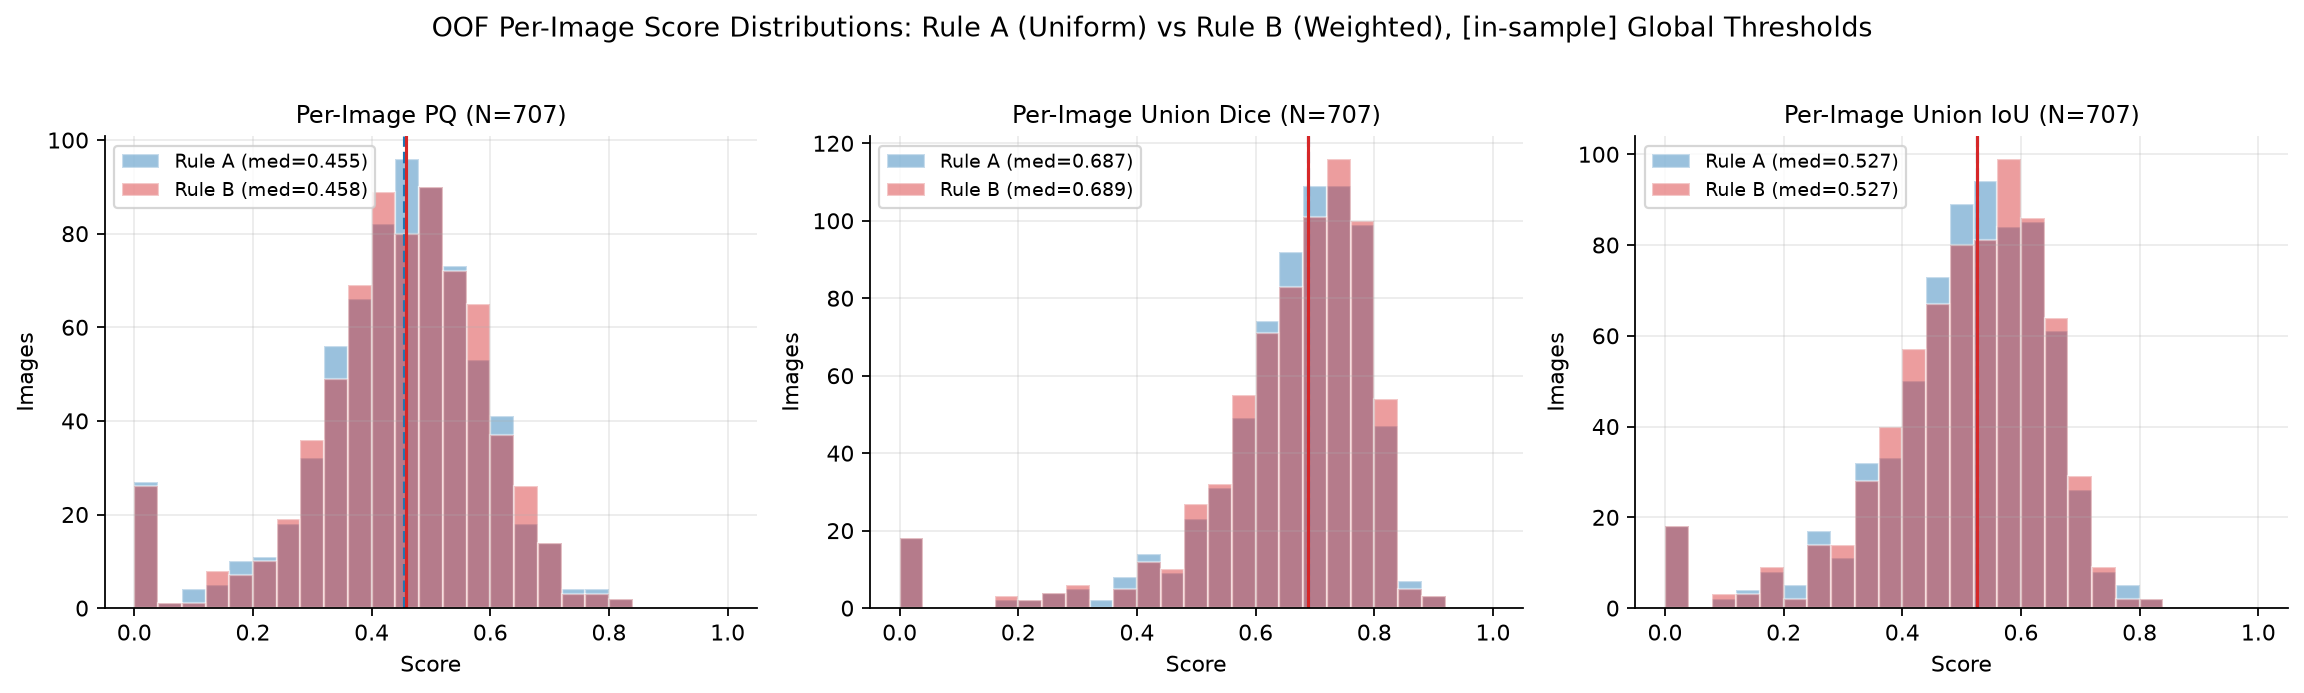
\includegraphics[width=\linewidth]{figures/oof_pq_dice_iou_distributions.png}
    \caption{OOF per-image PQ, Union Dice, and Union IoU distributions across all 707 training observations.}
    \label{fig:error_morph}
\end{figure}

\begin{figure}[t]
    \centering
    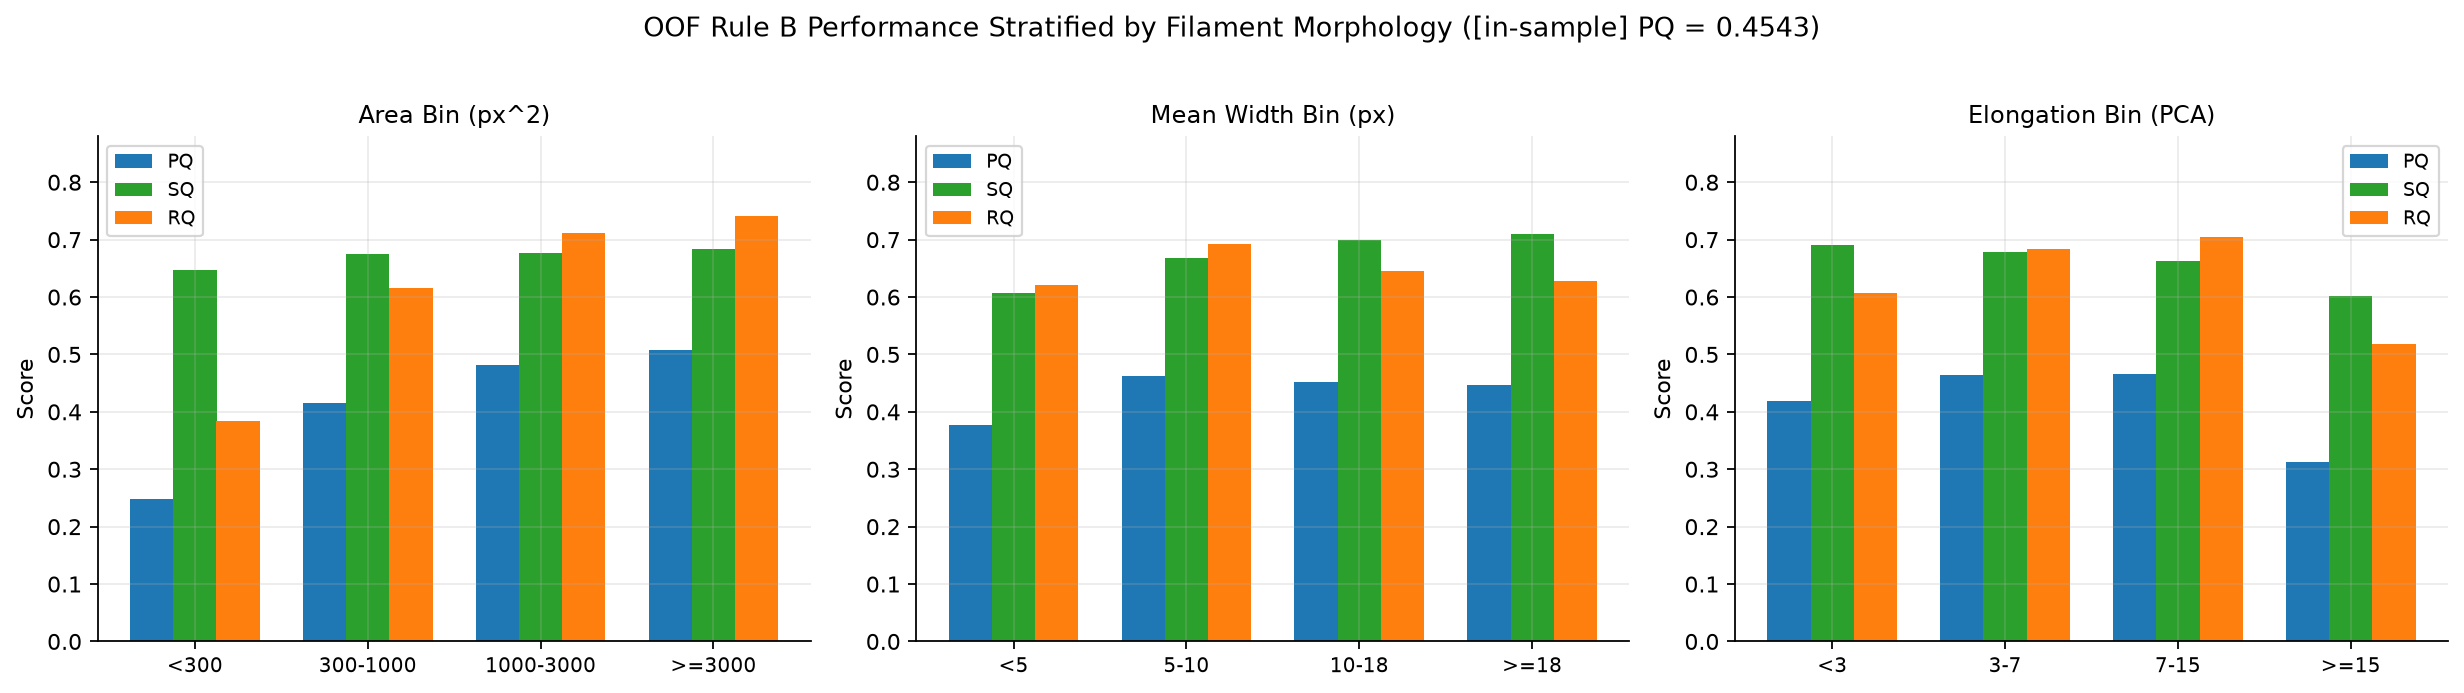
\includegraphics[width=\linewidth]{figures/morphology_stratified_pq.png}
    \caption{Stratified OOF Panoptic Quality by filament area, mean width, and PCA elongation.}
    \label{fig:morph_strat}
\end{figure}

\begin{figure}[t]
    \centering
    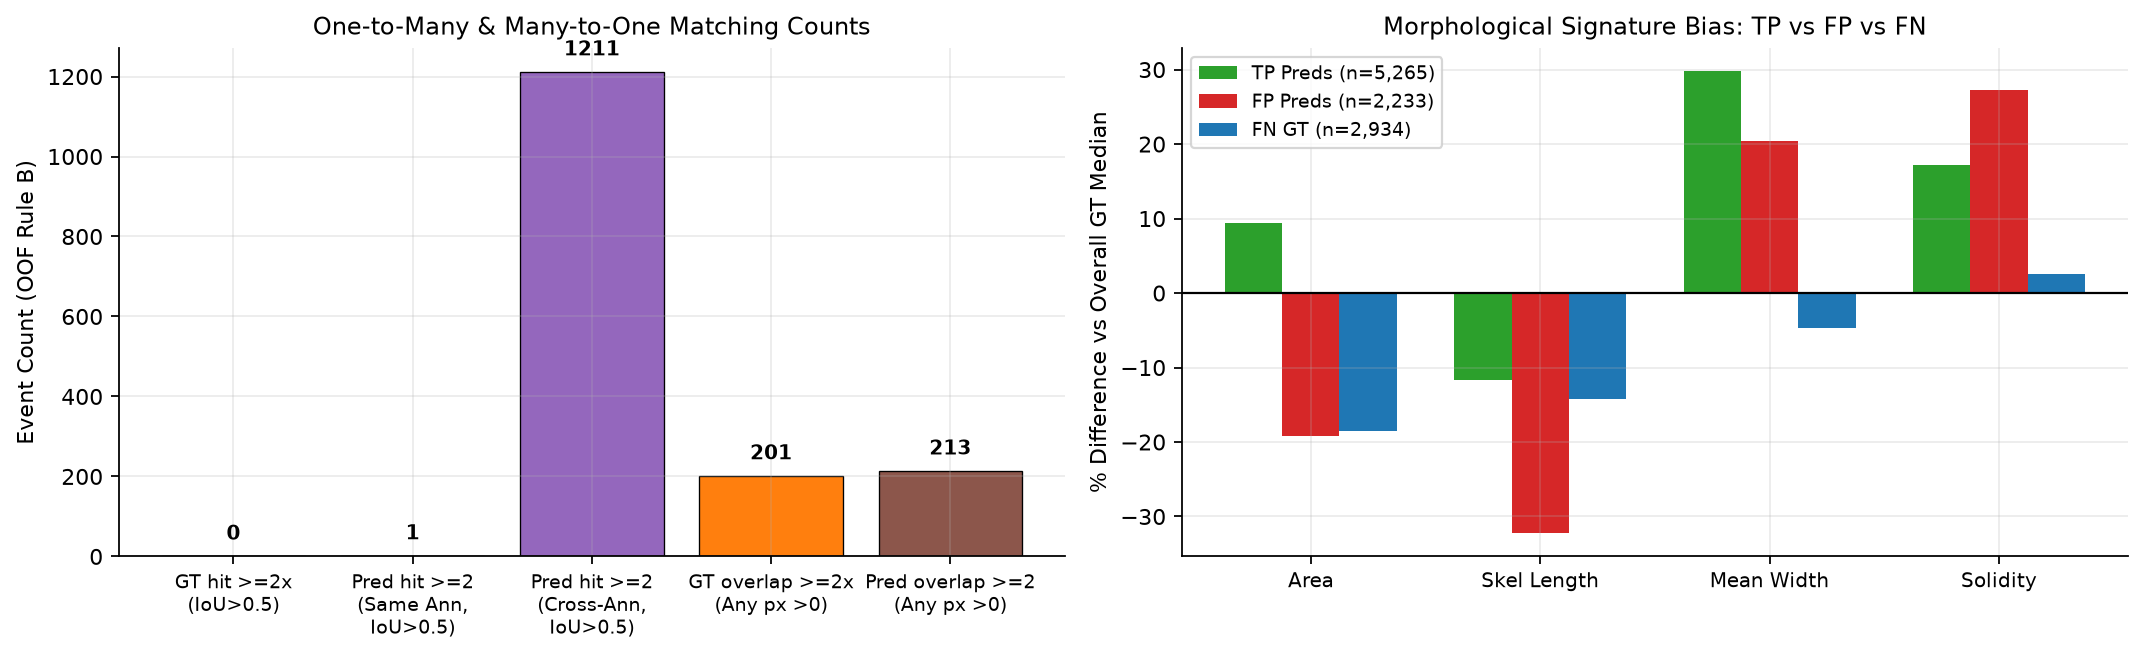
\includegraphics[width=\linewidth]{figures/matching_and_error_decomposition.png}
    \caption{One-to-one vs multi-hit matching counts and TP/FP/FN morphological signatures across 707 OOF observations.}
    \label{fig:matching_err}
\end{figure}

    \subsection{Failure Modes, Limitations \& Future Work}
    Morphological audit highlights sharp recall degradation on hyper-thin filaments ($\text{width} < 5\text{ px}$: PQ $0.3773$) and small regions ($\text{area} < 300\text{ px}^2$: PQ $0.2483$), whereas large filaments reach PQ $0.5072$. Multi-component predicted masks (5.71\% in OOF vs 0.37\% in GT) contribute concentrated False Positives ($\text{PQ}=0.1021$), and switching GT rasterization from official \texttt{frPyObjects} to \texttt{cv2.\allowbreak fillPoly} shifts nested 5-family PQ by $+0.0152$--$+0.0178$ ($0.4531 \rightarrow 0.4683$ and $0.4471 \rightarrow 0.4649$). Finally, single-annotator ground truth across 180 test images induces per-image variance ($\text{std}=0.1494$ in Rule~B OOF) relative to pooled multi-annotator CV ($0.4521$ \texttt{[nested]} / $0.4543$ \texttt{[in-sample]} vs $0.40$ LB; \texttt{Rule C} $0.4688$ \texttt{[nested]} vs $0.41$ LB). Future gains center on native $2048^2$ \texttt{frPyObjects}-supervised anchor detectors (\texttt{ResNeXt101-\allowbreak FPN}) to recover undetected sub-$5\text{ px}$ threads directly.


% ==================================== %
%            ACKNOWLEDGMENT            %
% ==================================== %
\section{Acknowledgment}\label{sec:acknowledgment}
    % Do not change
    The organization of the Filament Segmentation Challenge 2026 is partially supported by the U.S. National Science Foundation (NSF) under Grant No. 2209912 and 2433781, directorate for Computer and Information Science and Engineering (CSE), and Office of Advanced Cyberinfrastructure (OAC), and Grant No. 2511630, AST Division Of Astronomical Sciences and MPS Directorate for Mathematical and Physical Sciences.

    The Filament Segmentation Challenge 2026 is sponsored by the U.S. National Science Foundation (NSF) National Solar Observatory (NSO). 

    This work utilizes GONG data obtained by the NSO Integrated Synoptic Program, managed by the National Solar Observatory, which is operated by the Association of Universities for Research in Astronomy (AURA), Inc. under a cooperative agreement with the National Science Foundation and with contribution from the National Oceanic and Atmospheric Administration. The GONG network of instruments is hosted by the Big Bear Solar Observatory, High Altitude Observatory, Learmonth Solar Observatory, Udaipur Solar Observatory, Instituto de Astrofísica de Canarias, and Cerro Tololo Interamerican Observatory.

\bibliographystyle{ACM-Reference-Format}
\bibliography{main}

\end{document}
